\documentclass{article}

\usepackage{graphicx}
\usepackage{tikz}
\usepackage{tikzsymbols}
\usetikzlibrary{calc,patterns,shapes.geometric}
\pagestyle{empty}
\usepackage[margin=0pt]{geometry}
\geometry{papersize={14in,12in}}

\def\centerarc[#1](#2)(#3:#4:#5){\draw[#1] ($(#2)+({#5*cos(#3)},{#5*sin(#3)})$) arc (#3:#4:#5);}

\begin{document}
	\begin{figure}
		\centering
		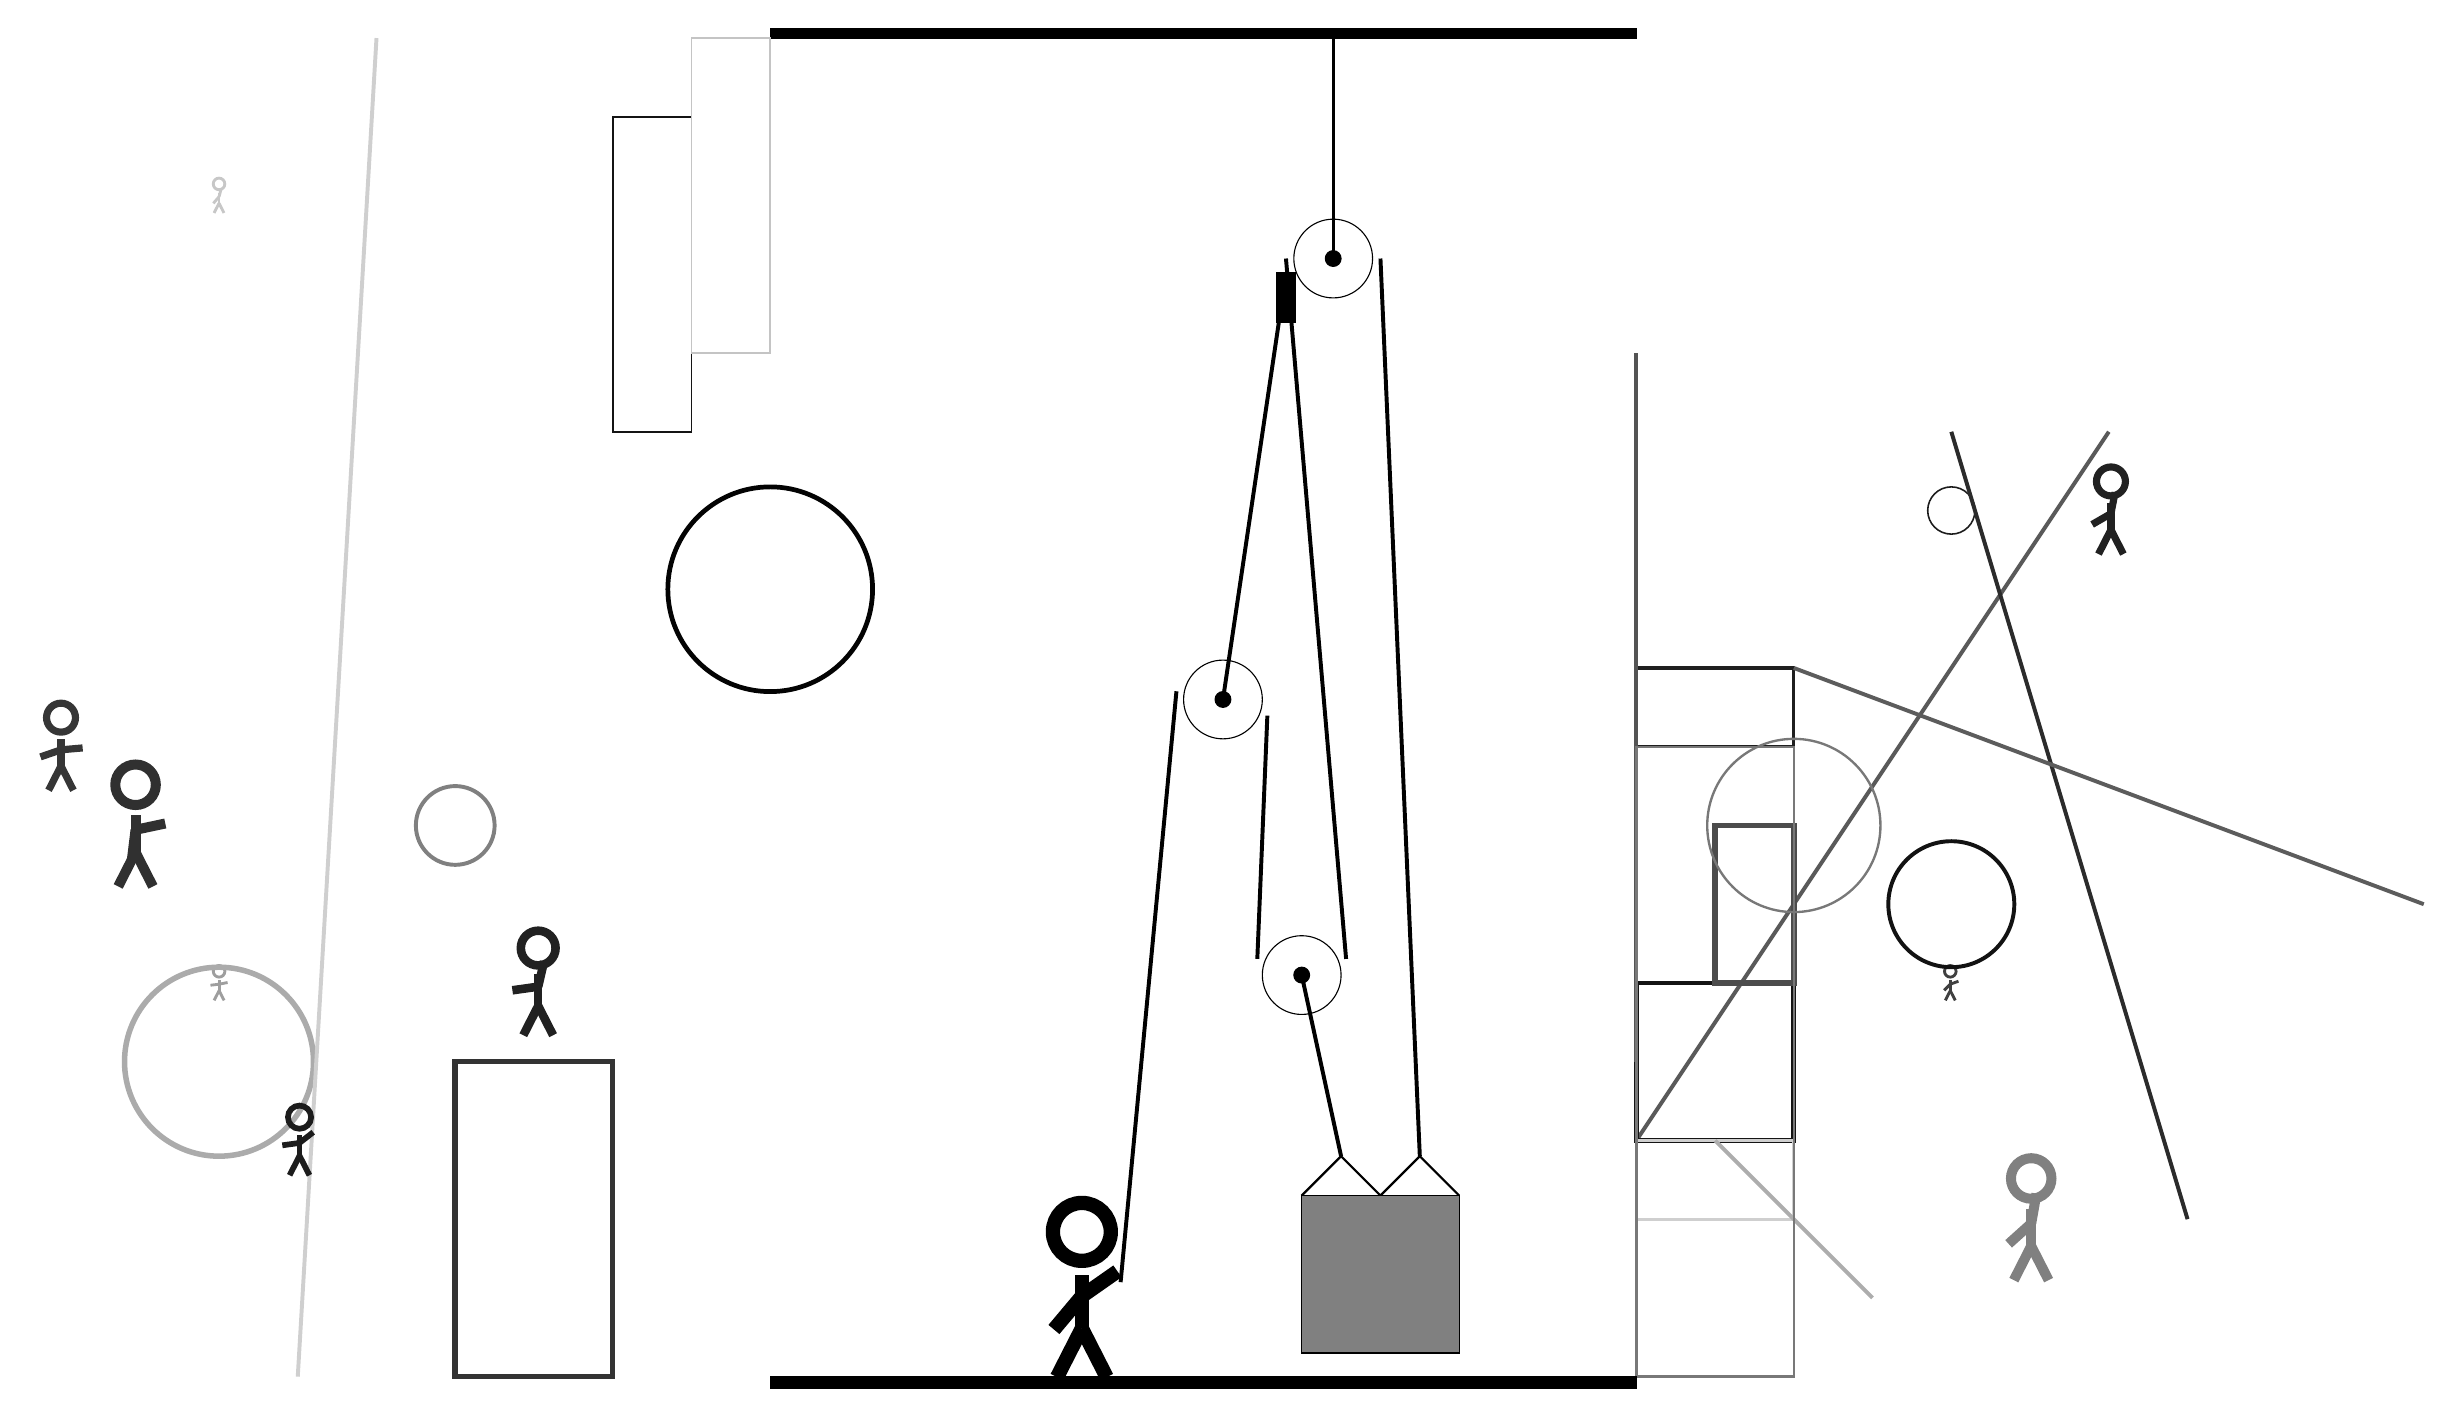
\begin{tikzpicture}
			%%%%% START %%%%%
			
			\draw[fill=black] (-6, 14) rectangle (5, 14.125);
			
			\draw (-0.25, 5.6) circle (0.5);
			\draw[fill=black] (-0.25, 5.6) circle (0.1);
			
			\draw[line width=0.5mm, color=black!65](5, 0) -- (11, 9);
			
			\node[line width=0.7mm, color=black!75] at (9, 2) {\Strichmaxerl[2][45][20]};
			\draw [line width=0.5mm, color=black!93](9, 3) circle (0.8);
			\node[line width=0.2mm, color=black!38] at (-13, 2) {\Strichmaxerl[2][7][11]};
			\node[line width=0.7mm, color=black!81] at (-14, 4) {\Strichmaxerl[7][83][12]};
			\draw [line width=0.2mm, color=black!89](9, 8) circle (0.3);
			\draw[line width=0.6mm, color=black!92] (7, 2) rectangle (5, 0);
			\draw [line width=0.5mm, color=black!50](-10, 4) circle (0.5);
			\node[line width=0.5mm, color=black!50] at (10, -1) {\Strichmaxerl[7][42][80]};
			\node[line width=0.6mm, color=black!87] at (-9, 2) {\Strichmaxerl[6][8][77]};
			
			\draw[line width=0.5mm, color=black!83](9, 9) -- (12, -1);
			
			\draw [line width=0.7mm, color=black!33](-13, 1) circle (1.2);
			\draw[line width=0.7mm, color=black!80] (-8, 1) rectangle (-10, -3);
			\draw[line width=0.5mm, color=black!19](-11, 14) -- (-12, -3);
			\node[line width=0.5mm, color=black!87] at (11, 8) {\Strichmaxerl[5][30][79]};
			\draw[line width=0.4mm, color=black!19] (5, -1) rectangle (7, 0);
			
			\draw[line width=0.4mm, color=black!88] (5, 5) rectangle (7, 6);
			\draw[line width=0.5mm, color=black!64](7, 6) -- (15, 3);
			\draw[line width=0.7mm, color=black!70] (6, 4) rectangle (7, 2);
			
			\node[line width=0.7mm, color=black!79] at (-15, 5) {\Strichmaxerl[5][19][5]};
			\draw [line width=0.3mm, color=black!53](7, 4) circle (1.1);
			\draw[line width=0.2mm, color=black!92] (-8, 9) rectangle (-7, 13);
			
			\node[line width=0.2mm, color=black!89] at (-12, 0) {\Strichmaxerl[4][8][38]};
			\draw[line width=0.2mm, color=black!23] (-6, 10) rectangle (-7, 14);
			\draw[line width=0.5mm, color=black!32](6, 0) -- (8, -2);
			
			\node[line width=0.7mm, color=black!22] at (-13, 12) {\Strichmaxerl[2][49][75]};
			
			\draw [line width=0.6mm, color=black!99](-6, 7) circle (1.3);
			\draw[line width=0.5mm, color=black!67](5, 1) -- (5, 10);
			\draw[line width=0.3mm, color=black!53] (7, 5) rectangle (5, -3);
			
			
			\draw (0.75, 2.1) circle (0.5);
			\draw[fill=black] (0.75, 2.1) circle (0.1);
			
			\draw (1.15, 11.2) circle (0.5);
			\draw[fill=black] (1.15, 11.2) circle (0.1);
			\draw[very thick] (1.15, 11.2) -- (1.15, 14);
			
			\draw[thick]  (0.75, -0.7) -- (1.25, -0.2) -- (1.75, -0.7) -- (2.25, -0.2) -- (2.75, -0.7);
			\draw[fill=black!50] (0.75, -0.7) rectangle (2.75, -2.7);
			
			\draw[line width=0.5mm] (-0.25, 5.6) -- (0.55, 11.0);
			\draw[line width=0.5mm, fill=black](0.45, 10.4) rectangle (0.65, 11.0);
			\draw[line width=0.5mm] (-1.55, -1.8) -- (-0.8409, 5.7042);
			\centerarc[line width=0.5mm](-0.25, 5.6)(-20:170:0.6);
			\draw[line width=0.5mm] (0.3138, 5.3948) -- (0.1862, 2.3052);
			\centerarc[line width=0.5mm](0.75, 2.1)(160:380:0.6);
			\draw[line width=0.5mm] (1.3138, 2.3052) -- (0.55, 11.2);
			\draw[line width=0.5mm](0.75, 2.1) -- (1.25, -0.2);
			\centerarc[line width=0.5mm](1.15, 11.2)(0:180:0.6);
			\draw[line width=0.5mm] (1.75, 11.2) -- (2.25, -0.2);
			
			\node at (-2, -1.9) {\Strichmaxerl[10][50][35]};
			
			\draw[fill=black] (-6, -3) rectangle (5, -3.15);
			
			%%%%% END %%%%%
		\end{tikzpicture}
	\end{figure}	
\end{document}